\documentclass{article}
\usepackage[utf8]{inputenc}
\usepackage[T1]{fontenc}
\usepackage{graphicx}	% images PNG
\usepackage{geometry}	% margins
\usepackage{url}		% links
\usepackage{charter}	% betterfont
\usepackage{stmaryrd}	% math symbols ?
\usepackage{eso-pic}
\usepackage{siunitx}	% SI units
\usepackage{amsmath}	% advanced math symbols
\usepackage{rotating}
\usepackage{multirow}	
\usepackage{color, colortbl}	% color fonts and table backgrounds
\usepackage{titlesec}
\usepackage{enumitem}
\usepackage{notoccite}
\usepackage{fancyhdr}	% page headers/footers
\newcommand\BackgroundPic{\put(0,0){\parbox[b][\paperheight]{\paperwidth}{
\vfill
\centering

\includegraphics[width=\paperwidth,height=\paperheight,keepaspectratio]{background.png}
\vfill
}}}
\geometry{top=1.5cm,bottom=1.5cm, left=2cm, right=2cm}
\titlespacing*{\paragraph}{0pt}{0pt plus 0pt minus 0pt}{0pt plus 0pt minus 0pt}
\titlespacing*{\subsection}{0pt}{0pt plus 0pt minus 0pt}{0pt plus 0pt minus 0pt}
\titlespacing*{\itemize}{0pt}{0pt plus 0pt minus 0pt}{0pt plus 0pt minus 0pt}

\title{Intermediate Work Report:}
\author{Louis Becquey}
\date{\today}

\setlength\parskip{\baselineskip}

\pagestyle{fancy}
\setlength{\headheight}{14.7pt}
\fancyhead[L]{\textsc{IP framework inserting RNA motives}}
% \fancyhead[L]{\leftmark}
\fancyhead[R]{Louis Becquey}
\fancyfoot[L]{}
\fancyfoot[C]{}
\fancyfoot[R]{\thepage}
\begin{document}

\begin{titlepage}
	\AddToShipoutPicture*{\BackgroundPic}
	\begin{center}
		\vspace{3cm}
		\LARGE
		\textsc{Intermediate Work Report:}\\
		{\Large Louis Becquey, \today}\\
		\vspace{2cm}
		\textit{An IP framework that uses detected possible RNA motifs\\ to predict RNA secondary structures}\\
	\end{center}
	\normalsize
	\vspace{5cm}
	
	\hrulefill
	\flushright{		
		\textbf{under the supervision of:\\}
			Fariza Tahi, HDR \\
			Eric Angel, HDR \\
			\textit{AROBAS, IBISC, Paris-Saclay University}\\
			~ \\
			
\includegraphics[height=1cm]{logoIBISC.png} ~ ~ 
			
\includegraphics[height=1cm]{minisaclay.png}
	}
	\flushleft
	\hrulefill
	\tableofcontents
\end{titlepage}
				
\newpage
\section{Motivation}
We now have quite consistent RNA motif databases (RNA3Dmotif \cite{djelloul_automated_2008}, the RNA Motif Atlas \cite{petrov_automated_2013}).\\
We call a RNA motif the combined description of these points:
\begin{itemize}
	\item A sequence or consensus sequence that we know to adopt a particular base-pairing organisation (sequence information),
	\item A particular base-pairing pattern in this sequence (or consensus sequence) considering canonical \& wobble pairing (bi-dimensional information),
	\item A particular organisation of non-canonical contacts in space (tri-dimensional information).
\end{itemize}
Then, a RNA motif is direct data about how a sequence can fold in space. Here, we are interested in using them to predict the bi or tri dimensional structure of an RNA sequence from scratch. 
Then, the algorithm we plan to use is the following:
	
\begin{itemize}
	\item Find all possible occurences of known RNA motifs in the query sequence by pattern matching of the motifs consensus sequences against the query bases,
	\item Define constraints on the secondary structure imposed by motives if included
	\item Find a secondary structure that satisfies both the most the expected accuracy (MEA model) and criterion of motif inclusion, by solving a bi-objective IP problem, using the previous constraints.
\end{itemize}

\newpage
\section{Pattern matching to detect motif sites}
A very complete model has been developped by the BGSU team \cite{zirbel_identifying_2015}, 
which perfectly suits this need: JAR3D finds, given a RNA sequence with no additional information, 
the sites that are likely to fold in known 3D motives of the RNA Motif Atlas \cite{petrov_automated_2013}.

The RNA 3D Motif Atlas is an updated database of substructures exracted from a non-redundant set of 3D RNA structures. They are grouped into "motifs", which are a given pattern of 3D non-canonical interactions.
Each motif contains one or several instances observed in real RNA structures. 
The instances might differ in sequence, length of bulged insertions, and other details, but share a common graph of 3D non-canonical interactions.

For each motif group of the database, JAR3D estimates the probability that a sequence folds into the 3D pattern, given the known members of the motif group. It takes into account crossed contacts, base-ribose and base-phosphate interactions, and triple base-pairs.

This is the most scientifically correct approach to use to my knowledge. Unfortunately, the code is in MatLab and seems hard to use on a single computer (JAR3D is basically a webserver).

\section{Formulation of the IP problem}
	
This formulation is an improved merge between the IPknot \cite{sato_ipknot:_2011} formulation (without "levels") and RNAMoIP's one \cite{reinharz_towards_2012}.
% This problem has been inspired by IPknot's model \cite{sato_ipknot:_2011}, but without the use of what they call \textit{levels}, which are pseudoknot-free
% structures that should be superposed to give the true pseudoknotted secondary structure graph.\\
% Levels are mutually exclusive (a base cannot be paired in two different levels). The more levels you use, the more decision variables you have, 
% but the more complex pseudoknots you are able to predict. IPknot and BiokoP use 2 levels, to predict simple knots.\\
% \begin{figure}[h]\centering 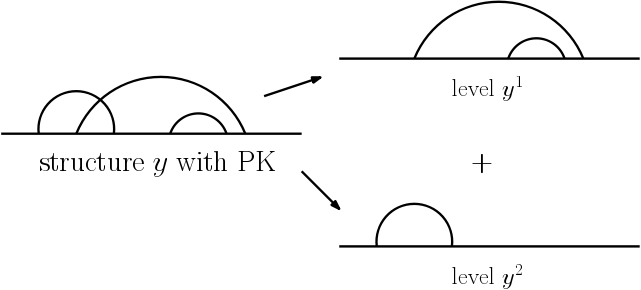
\includegraphics[height=5cm]{levels.png}\end{figure}
	
	
\subsection{Variables} 
	
% Let $m$ be the number of levels that our program uses.\\
Let $n$ be the number of nucleotides in the query RNA sequence $s$.\\
Let $M$ be the set of motifs that could be inserted in $s$ (a match exist between $s$ and the sequence of the motifs' components).\\
Let $x$ be a motif of $M$, $x$ having $j^x$ distinct components.\\
Let $P_{x,i}$ be the set of positions in $s$ where we can insert the $i$th component of motif $x$.\\
Let $k_{x,i}$ be the size in nucleotides of that $i$th component of $x$.\\
Let $y^u_v$ be the \textbf{decision boolean variable} indicating that $s[u]$ and $s[v]$ form a canonical base pairing. Then, we always have $u \neq v$.\\
Let $C^{x,i}_p$ be the \textbf{decision boolean variable} indicating that we do insert the $i$th component of motif $x$ at position $p$.
	
	
Note that a base pair $y^u_v$ is possible if and only if $v>u+3$, and that we do not need to use two variables $y^u_v$ and $y_{vu}$ for the same pair. 
Then, we have $\sum_{i=4}^n (n-i)$ decision variables ($\approx \frac{1}{2}n^2$ decision variables) of the form $y^u_v$.
Regarding the $C^{x,i}_p$, if we have an average insertion of $\nu$ motives by RNA sequence, the motives having in average $\mu$ components, components that can be inserted in average at $\pi$ different positions in $s$,
then we need to add, in average, $\nu \times \mu \times \pi$ decision variables $C^{x,i}_p$.

Then, we expect having around $\frac{1}{2}n^2+\nu \mu \pi$ decision variables.

\newpage
\subsection{Objectives}
We have two objectives : Find a structure with correct expected accuracy, and find a structure which includes (large) known motifs.
Let $X$ be the vector of all our decision variables, we define the following loss functions to maximize:
$$ f_1(X) = \sum_{x \in M} \left[ (j^x)^2 \times \sum_{p \in P_{x,1}} C^{x,1}_p \right]$$
$$ f_2(X) = \sum_{u<v} p_{uv}\times y^u_v \times I[p_{uv}>\theta], \qquad \qquad
p_{uv} = \sum_{\sigma \in S(s)} y^u_v.p(\sigma | s)$$
$f_1$ is supposed to maximize the number of inserted motives in $s$, weighted by their number of components.
$f_2$ is supposed to maximise the expected accuracy of the secondary structure (MEA model). 
$p_{uv}$ are the base pairing probabilities that can be estimated from a set $S(s)$ of secondary structures of $s$.

\subsection{10 Constraints to bind them all}
\paragraph{Constraint to ensure there only is 0 or 1 canonical pairing by nucleotide} ~ 
\begin{equation} \label{constraint:1}
	\sum_{v>u} y^u_v + \sum_{v<u} y^v_u \leq 1 \qquad\qquad \forall u \in \llbracket 1,n \rrbracket
\end{equation}
	
\paragraph{Constraints to forbid lonely base pairs} ~
\begin{equation} \label{constraint:2}
	1 + \sum_{v=u}^n y^{u-1}_v - \sum_{v=u+1}^n y^u_v + \sum_{v=u+2}^n y^{u+1}_v \geq 1 \qquad \qquad \forall u \in \llbracket 1,n\rrbracket
\end{equation}
\begin{equation} \label{constraint:3}
	1 + \sum_{u=1}^{v-2} y^u_{v-1} - \sum_{u=1}^{v-1} y^u_v + \sum_{u=1}^{v} y^u_{v+1} \geq 1 \qquad \qquad \forall v \in \llbracket 1,n\rrbracket
\end{equation}
These conditions ensure that if a base pair exists with $s[i]$, 
one of the adjacent bases is paired too. 
Equation \ref{constraint:2} is useful if $s[u]$ is paired with $s[v>u]$ (a nucleotide later in the sequence), 
and equation \ref{constraint:3} if $s[v]$ is paired with $s[u<v]$ (a nucleotide earlier in the sequence).
	
\paragraph{Constraint to forbid pairings inside a motif component} ~ 
\begin{equation} \label{constraint:4}
	k_{x,i} \; C^{x,i}_p + \sum_{u=p}^{p+k_{x,i}-1}\left[ \sum_{v>u} y^u_v + \sum_{v<u} y^v_u \right] \leq k_{x,i} 
	\qquad \qquad \forall p \in P_{x,i} \qquad \forall x \in M, i \in \llbracket 1,j^x \rrbracket
\end{equation}
	
\paragraph{Constraint to forbid component to overlap} ~
\begin{equation} \label{constraint:5}
	\sum_{x \in M} \sum_{i=1}^{j^x}\sum_{\substack{p \in P_{x,i}\\u-k_{x,i}+1 \leq p \leq u}}^u C^{x,i}_p \leq 1 \qquad \qquad \forall u \in \llbracket 1,n \rrbracket
\end{equation}
Then, whatever the nucleotide $u$, it can be part of a motif component only once. 
$u$ belongs to a component $x,i$ if and only if $u-k_{x,i}+1 \leq p_{x,i} \leq u$.\\
\begin{center}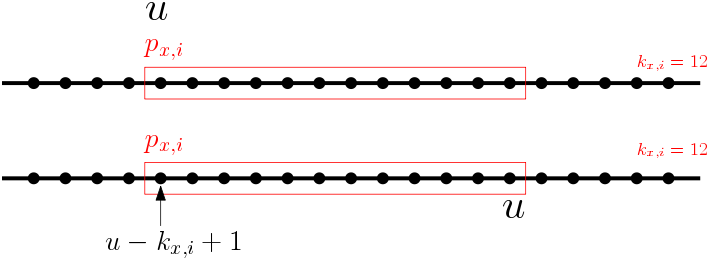
\includegraphics[height=3cm]{component.png}\end{center}
	
\paragraph{Constraints to respect the structure of large motives ($\forall x \in \{ x\in M | j^x \geq 2\}$)} ~ 

The first two constraints ensure that a component is inserted if and only if the next and the previous one are also inserted somewhere.
They also force a minimal distance of 3 nucleotides between any two consecutive components of the same motif.
\begin{equation}\label{constraint:6}
	C^{x,i}_p \leq \sum_{\substack{p' \in P_{x,i+1}\\ p'>p+k_{x,i}+2}} C^{x,i+1}_{p'}	
	\qquad \qquad \forall p \in P_{x,i} \qquad \forall x \in \{ x\in M | j^x \geq 2\}, i \in \llbracket 1,j^x \llbracket
\end{equation}
\begin{equation}\label{constraint:7}
	C^{x,i}_p \leq \sum_{\substack{p' \in P_{x,i-1}\\ p'<p-k_{x,i-1}-2}} C^{x,i-1}_{p'}	
	\qquad \qquad \forall p \in P_{x,i} \qquad \forall x \in \{ x\in M | j^x \geq 2\}, i \in \rrbracket 1,j^x \rrbracket
\end{equation}
We add another one to ensure that all components of any motif are inserted the same number of times in $s$:
\begin{equation}\label{constraint:8}
	\sum_{p\in P_{x,1}} C^{x,1}_p - \frac{1}{j^x} \sum_{i=1}^{j^x} \sum_{p\in P_{x,i}} C^{x,i}_p = 0  \qquad \qquad x\in M
\end{equation}
And finally, we force base pairs between the end of a component and the beginning of the next one:
\begin{equation}\label{constraint:9}
	C^{x,i}_p \leq \sum_{p' \in P_{x,i-1}} y^{p'+k_{x,i}-1}_p \qquad \qquad \forall x \in \{ x\in M | j^x \geq 2\}, i \in \rrbracket 1,j^x \rrbracket
\end{equation}
\begin{equation}\label{constraint:10}
	C^{x,i}_p \leq \sum_{p' \in P_{x,i+1}} y^{p+k_{x,i}-1}_{p'} \qquad \qquad \forall x \in \{ x\in M | j^x \geq 2\}, i \in \llbracket 1,j^x \llbracket
\end{equation}

\section{Remaning questions}
	\begin{itemize}
		\item I am not sure how to compute the base-pair probabilities for the MEA model (objective $f_2$). 
		If you already have a set of secondary structures $S(s)$, why do you need this program ?
		\item In objective $f_1$, weighting the motif by the number of components (squared) shows no reason to be the best idea. 
		Some exploration is needed. An additional weight given by the pattern-matching step might be an idea, reflecting the probability to see the motif here in $s$.
		
	\end{itemize}
	
%%%%%%%%%%%%%%%%%%%%%%%%%%%%%%%%%%%%%%%%%%%%%%%%%%%%%%%%%%%%%%%%%%%%%%%%%%%%%%%%%%%%%%%%%%%%%%%%%%%%%%
% \newpage
\bibliographystyle{unsrt}
\bibliography{RNA}
\end{document}